\section{Impact of charging station placement}
\label{sec:6_5_freefloating}

\subsection{Simulation setup}
In this section I run several accurate simulation through the simulator described in chapter \ref{chap:5_simulator}. More in detail, for each city, I built the trace replicating the start and end for each rentals, with a fleet size reported in table \ref{tab:6_summary}. Those particular simulation deeply studied the pro and cons of different provider settings like charging stations placement and car return policy.

In particular, the main provider side performances is the percentage of \textit{infeasible trips} (trips where the battery completely run out before to reach the destination). From an user point of view, I measure the \textit{discomfort metrics}, the metrics that may be seen as extra work from the user side. They namely are the \textit{charge events}, \textit{percentage of reroutings}, \textit{average plug time} and the \textit{average walking distance}. 

The best configuration is the one that makes the \textit{infeasible trips} close to 0\% and minimizes all the others metrics.

\subsection{Results}

I consider, initially,  the Free Floating return policy (described in section\ref{sec:5_4_return_policy}), and I study the impact different charging station placement policies. The aim is to check what would be the minimum number of charging stations to install to sustain a FFCS system based on electric vehicles that is equivalent to the one currently in use.

\begin{figure*}[t!]
	\begin{center}
		
\includegraphics[width=\textwidth]{figures/legenda2.pdf}
	\end{center}
	\begin{center}
		\begin{subfigure}{0.49\textwidth}
			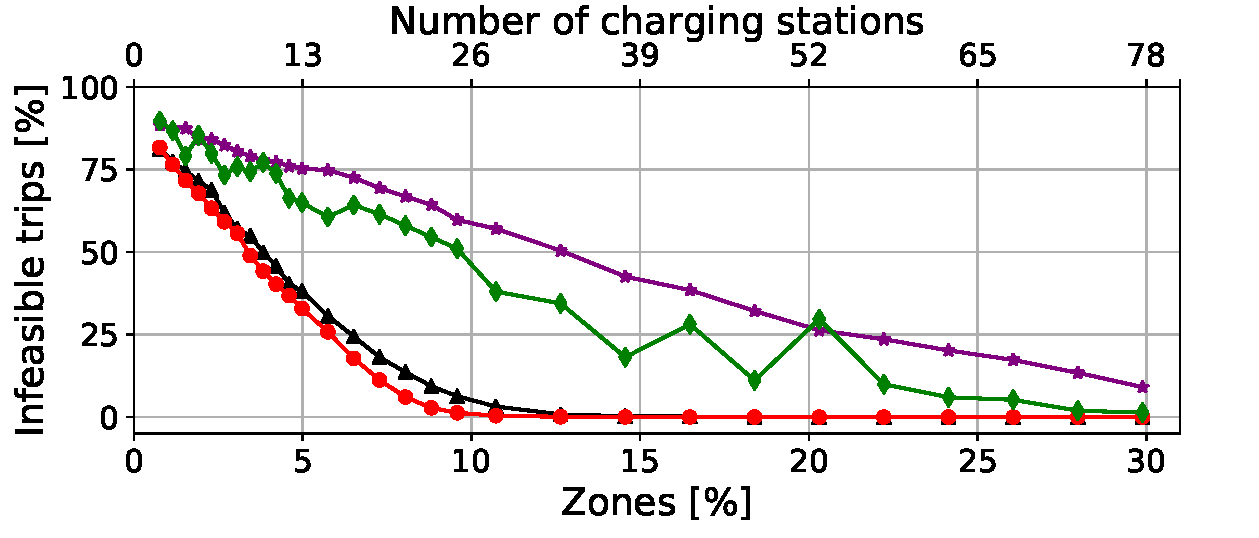
\includegraphics[width=\columnwidth]{figures/Torino_zonesVsDeaths_algorithms_acs-4_tt-25_policy-FreeFloating.pdf}
			\caption{Turin}
			\label{fig:6_4_zone_vs_deaths_torino}
		\end{subfigure}
		\begin{subfigure}{0.49\textwidth}
			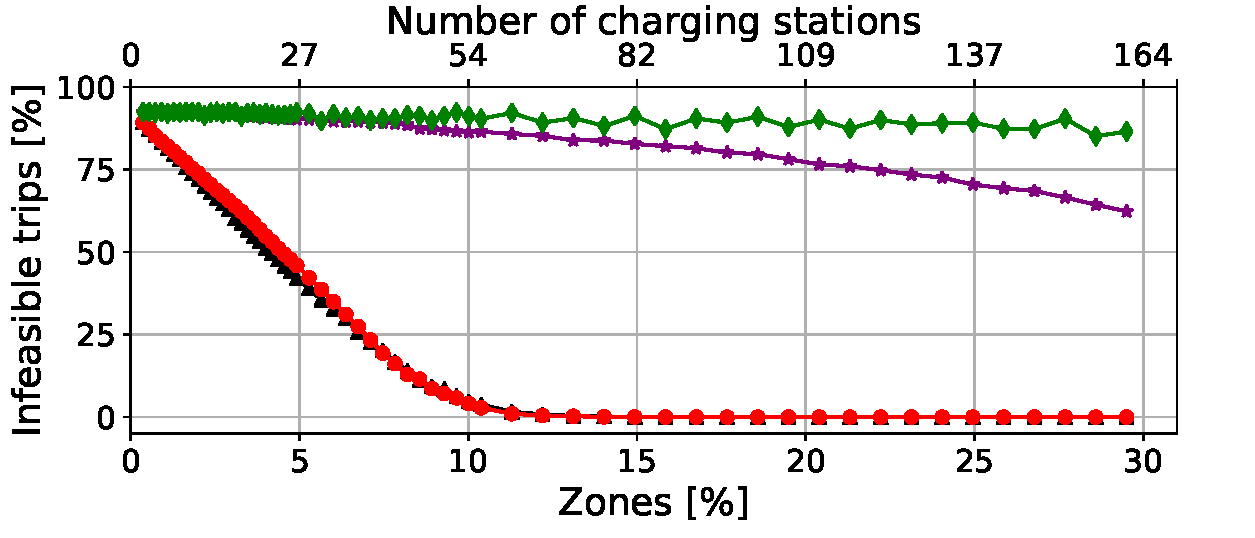
\includegraphics[width=\columnwidth]{figures/Milano_zonesVsDeaths_algorithms_acs-4_tt-25_policy-FreeFloating.pdf}
			\caption{Milan}
			\label{fig:6_4_zone_vs_deaths_milano}
		\end{subfigure}
		\begin{subfigure}{0.49\textwidth}
			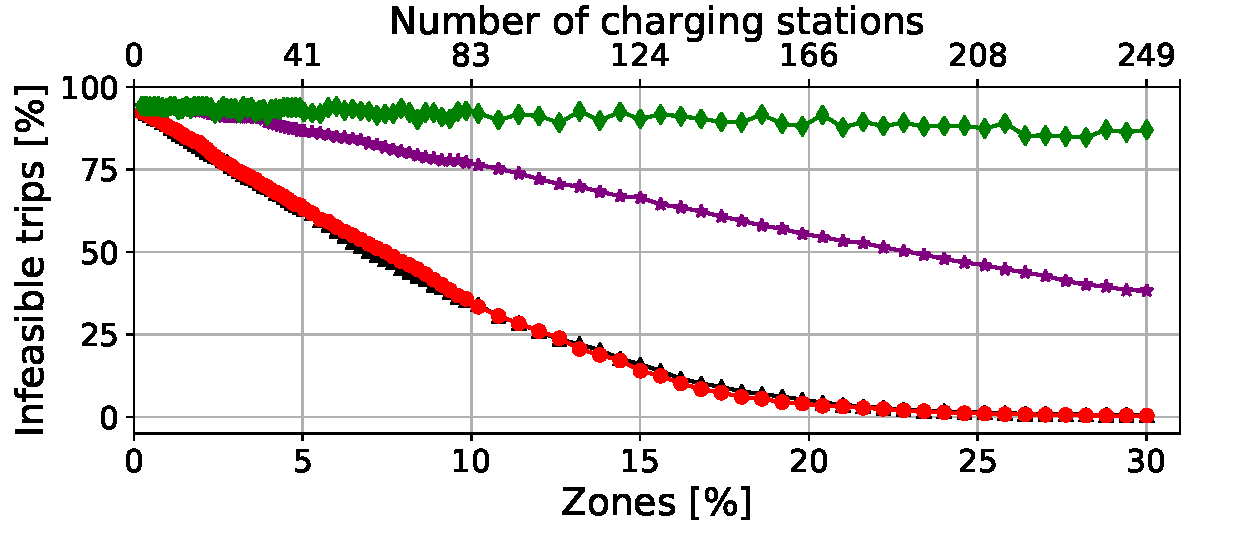
\includegraphics[width=\columnwidth]{figures/Berlino_zonesVsDeaths_algorithms_acs-4_tt-25_policy-FreeFloating.pdf}
			\caption{Berlin}
			\label{fig:6_4_zone_vs_deaths_berlino}
		\end{subfigure}
		\begin{subfigure}{0.49\textwidth}
			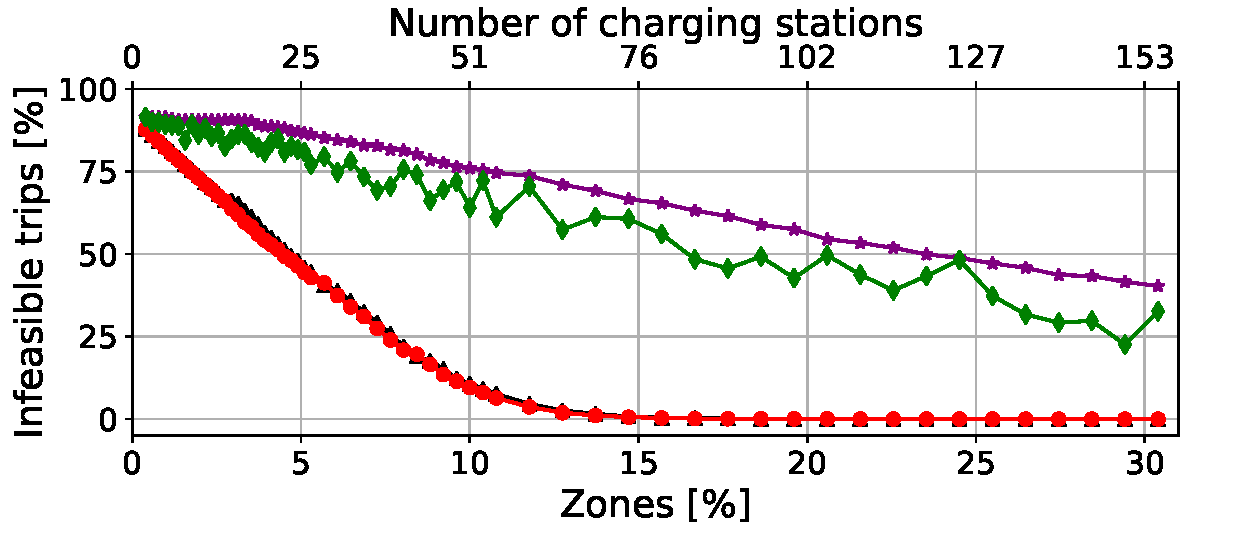
\includegraphics[width=\columnwidth]{figures/Vancouver_zonesVsDeaths_algorithms_acs-4_tt-25_policy-FreeFloating.pdf}
			\caption{Vancouver}
			\label{fig:6_4_zone_vs_deaths_vancouver}
		\end{subfigure}         
		\caption{Percentage of unfeasible trips as function of charging station number, for different placement algorithms and city. Placing charging stations where cars are frequently parked is much better than where cars stay parked for long time.}
		\label{fig:6_4_deathsVsZones_algorithm}
	\end{center}
\end{figure*}


Figure~\ref{fig:6_4_deathsVsZones_algorithm} shows the performance of the different placement algorithms in terms of percentage of infeasible trips  with respect to  the number of charging stations $N$ for each city. Each charging station has $k=4$ poles. Bottom x-axis reports the percentage of equipped zones with respect to the total, while top x-axis reports the actual number, different for each city.

It is possible observe notably different performance for different placement algorithm. First, the average parking time placement policy (\textit{Avg time} - purple line) has very poor performance in all the cities. Even a simple random choice sometimes performs better (\textit{Mean rnd} - green line, obtained as the average of 10 random instances). However, in Milan -- figure.~\ref{fig:6_4_zone_vs_deaths_milano} -- and Berlin -- figure~\ref{fig:6_4_zone_vs_deaths_berlino}, the random placement results the worst. This is due to the larger number of zones, which makes the space of available solutions much larger.

Second, the total parking time  (\textit{Tot time} - black line) and total number of parkings (\textit{Num parking} - red line) perform similarly and consistently better than other policies. A 10\% coverage in Turin, 11\% in Milan, 23\% in Berlin\%, and 13\% in Vancouver lead to about 2\% of infeasible trips. 
In all the city but Berlin it is possible to reach a negligible percentage of infeasible trips with just 15-18\% of charging zones. Instead, in Berlin it is possible still have some infeasible trips with 30\% of charging zones. Recalling that with the designed it is possible travel 135\,km \ref{sec:5_5_kpi_scenario}, the presence of infeasible trip is explained by looking the rental distance presented in~\ref{fig:cdf_characterization}. Trips in Berlin can be as long as 39\,km. Therefore, with only 4 long-trips which do not end in a charging station area, the battery could run out the energy.

The overall trends confirm the intuition of why the recharging stations placement algorithm is of primary importance. \textit{Avg time} placement favours peripheral zones where few trips end, and where cars stay parked for long time, sometime longer than the time required for a complete charge, (see left heat maps~figure~\ref{fig:heatmap_Berlin} and figure~\ref{fig:heatmap_vancouver}). On the contrary, \textit{Num parking} and \textit{Tot time} favour city center areas, where cars are frequently parked for short time (see right heat maps in ~figure~\ref{fig:heatmap_Berlin} and figure~\ref{fig:heatmap_vancouver}). 

Figure \ref{fig:7_6_CDF_parking_time_per_algorithm} confirms this intuition. Indeed the \textit{Avg time} placement generates much longer plugged times, often much longer than the time needed for a full charge. Therefore, many cars occupy the charging poles when they are already charged, preventing other cars to use those poles and increasing the number of infeasible trips. 

\begin{figure}[ht]
	\centering
	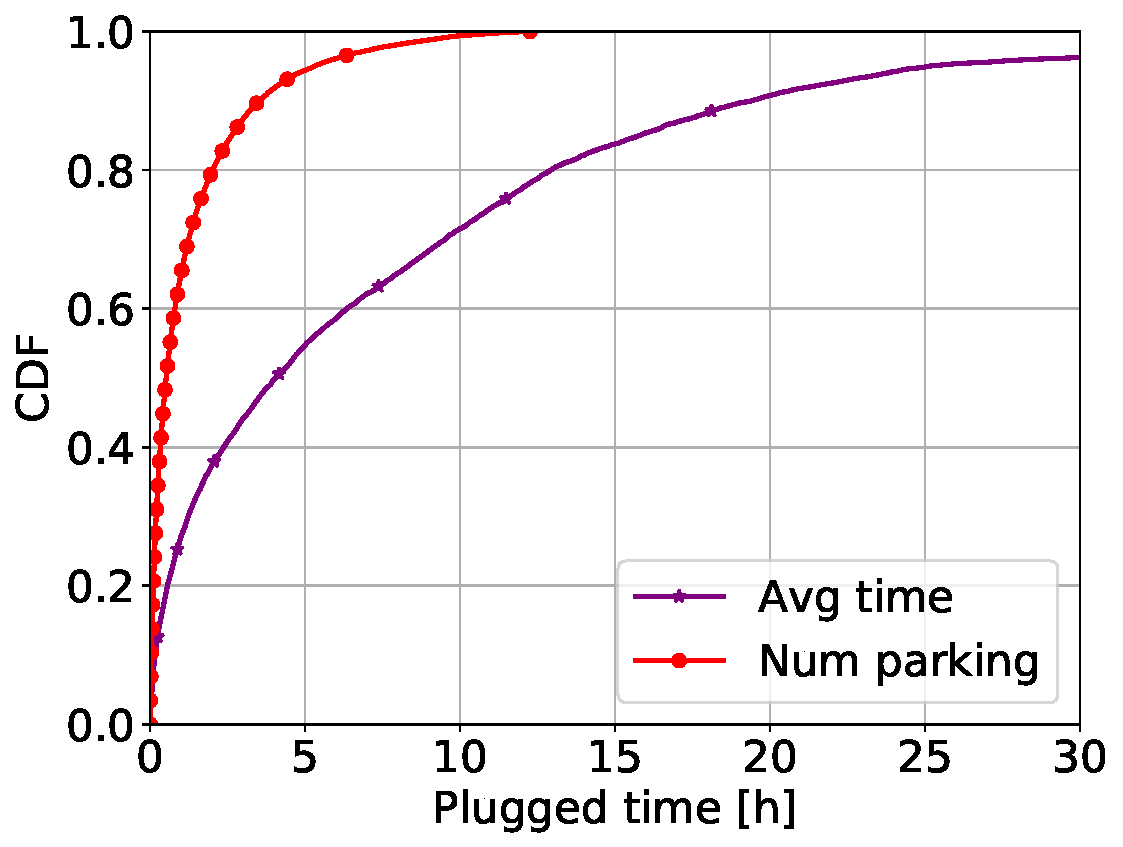
\includegraphics[width=0.5\columnwidth]{figures/CDF_parking_time_per_algorithm.pdf}
	\caption{CDF of the time spent by a car at a charging station (Z=40), for \textit{Num parking} and \textit{Avg time} placement algorithms in Turin. }
	\label{fig:6_6_CDF_parking_time_per_algorithm}
\end{figure}



\textbf{Takeaway:} Placing charging stations in areas where cars stay parked for long time is not convenient. Placing charging stations in areas which allow many cars to recover the (little) energy consumed in the (short) trips results in a much better policy.

Given this, the total number of parking is the placement algorithm and it will be used for the rest of the chapter. 

